\chapter{DESIGN AND MODELING}

Design and modeling are essential phases in the software development lifecycle, playing a
crucial role in the creation of effective and wellstructured systems. These phases involve
the conceptualization, planning, and representation of a software solution before its actual
implementation.
\section{Activity Diagram}
An activity diagram is a type of UML (Unified Modeling Language) diagram that visually represents the flow of activities in a system or business process. It is commonly used in software development to illustrate the dynamic aspects of a system and describe how different activities or tasks interact with each other. Activity diagrams are particularly useful for modeling the workflow within a system and for understanding the sequence of actions that take place.

\subsection{Key elements of Activity Diagrams}
\begin{itemize}
    \item \textbf{Activity:} Represented by rounded rectangles, activities are the specific tasks or actions that are performed within the system. These can range from simple operations to complex processes.
    \item \textbf{Transitions:} Arrows connecting activities indicate the flow or transition from one activity to another. The direction of the arrow shows the order of execution.
    \item \textbf{Decision Nodes:} Diamonds are used to represent decision points in the workflow. Depending on certain conditions, the process may take different paths.
    \item \textbf{Fork and Join Nodes:} Fork nodes (split) and join nodes (merge) show parallel or concurrent activities. Forks represent the divergence of multiple flows, while joins represent their convergence.
    \item \textbf{Initial and Final Nodes:} Circles are used to denote the start (initial node) and end (final node) of the activity diagram. The initial node represents the beginning of the process, and the final node indicates the conclusion.
\end{itemize}


\begin{figure}[H]
    \centering
    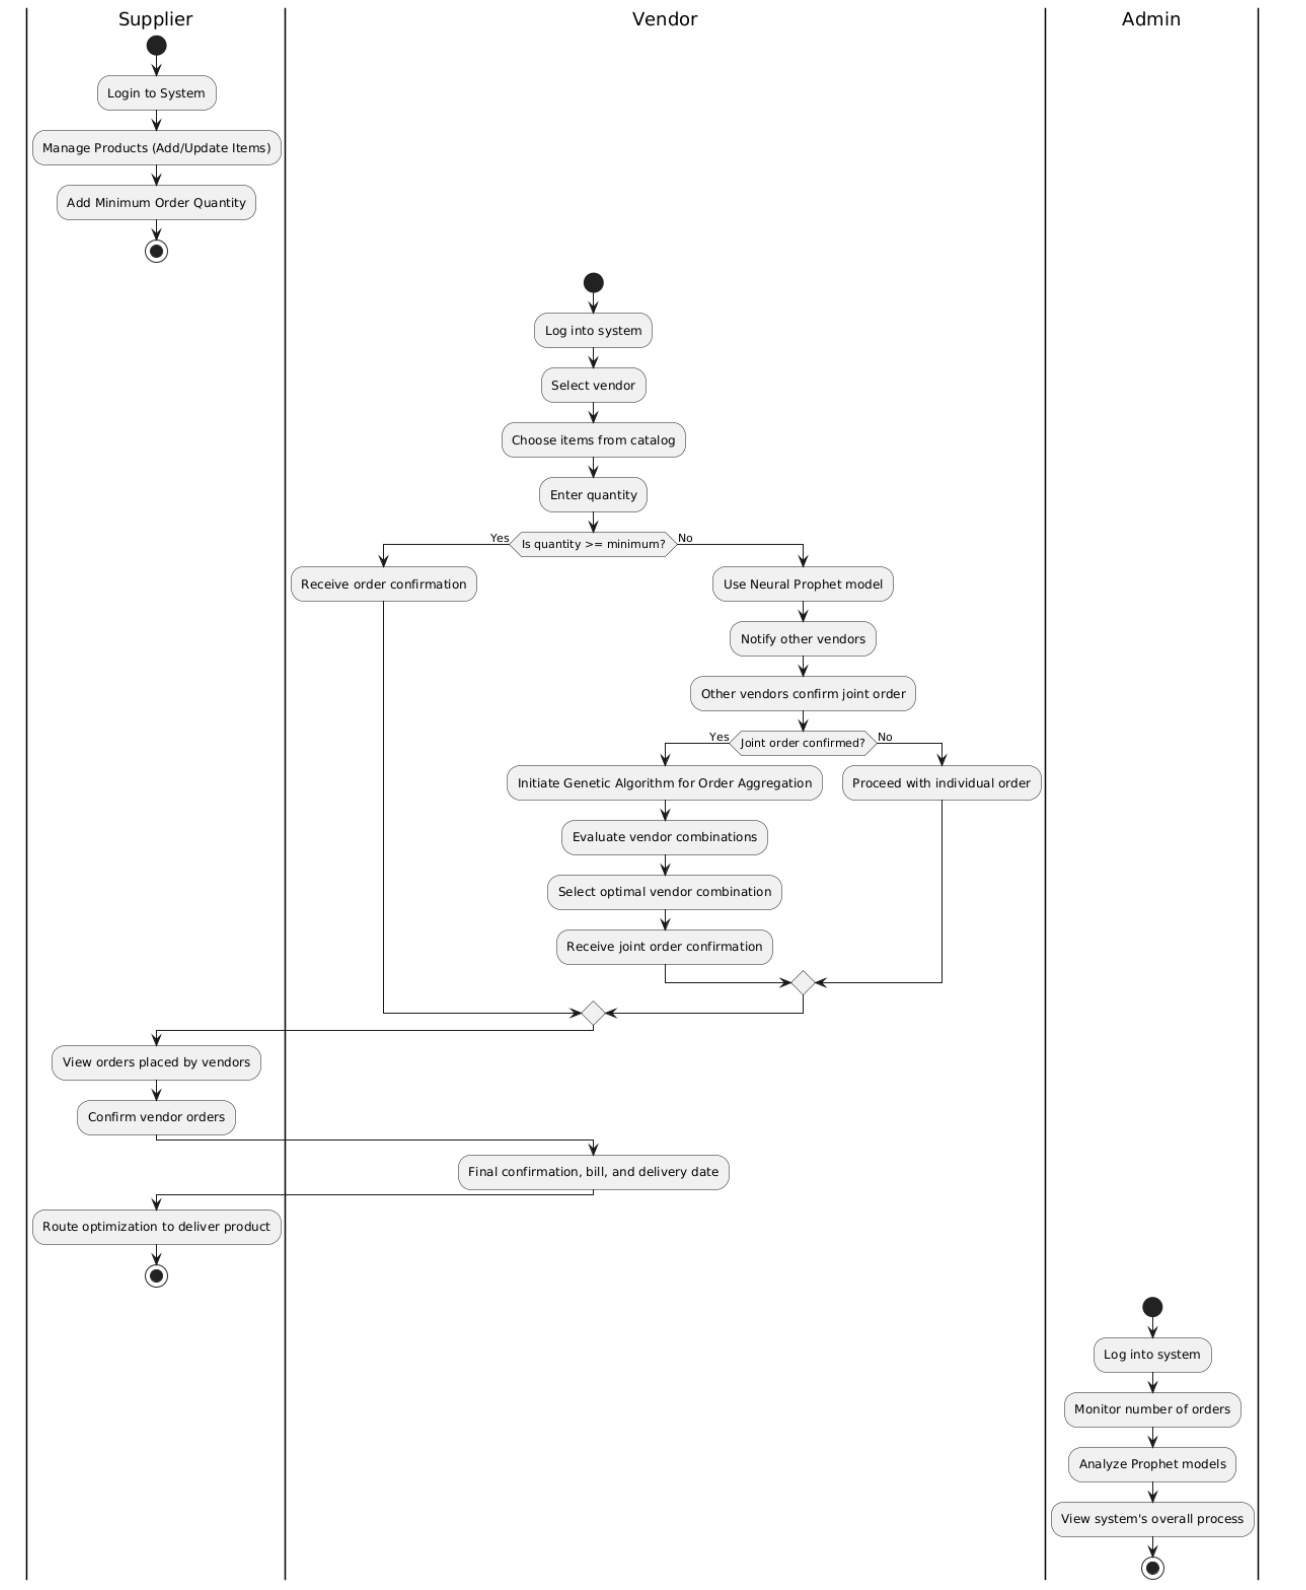
\includegraphics[width=0.9\textwidth]{Figures/Activity diagram.jpeg}
    \caption{Activity Diagram}
    \label{fig:activity-diagram}
\end{figure}
\noindent Figure 4.1 illustrates the activity diagram for the ASTRO Platform, showcasing the sequence of activities performed by suppliers, vendors, and admins. This diagram provides a high-level overview of the key entities and components involved in the system, detailing their interactions and responsibilities throughout the order processing and delivery process.

\subsection{Key Entities and Components}
\begin{enumerate}
    \item \textbf{Supplier Activities}
          \begin{enumerate}
              \item \textbf{Login to System:} The supplier logs into the system to access functionalities for managing products and tracking orders.
              \item \textbf{Manage Products (Add/Update Items):} Suppliers add or update product listings to ensure the catalog is up-to-date and accurate.
              \item \textbf{Add Minimum Order Quantity:} Suppliers set a minimum order quantity for each product, preventing inefficient processing of very small orders.
              \item \textbf{View Orders Placed by Vendors:} Suppliers can view pending orders from vendors, preparing them for order fulfillment.
              \item \textbf{Confirm Vendor Orders:} Suppliers review and confirm vendor orders, moving them to the fulfillment phase.
              \item \textbf{Route Optimization for Delivery:} The supplier optimizes delivery routes to reduce logistics costs and ensure timely product delivery.
          \end{enumerate}

    \item \textbf{Vendor Activities}
          \begin{enumerate}
              \item \textbf{Log into System:} Vendors start by logging into the system to access the product catalog and ordering functionalities.
              \item \textbf{Select Vendor and Choose Items from Catalog:} Vendors select suppliers to order from, browsing the catalog to choose items.
              \item \textbf{Enter Quantity:} Vendors input desired quantities for each item, triggering a check against the minimum order quantity.
              \item \textbf{Quantity Check (Yes/No):}
                    \begin{itemize}
                        \item \textbf{If Quantity Meets Minimum Requirement:} The order is confirmed directly.
                        \item \textbf{If Quantity Is Below Minimum Requirement:}
                              \begin{enumerate}
                                  \item \textbf{Use Neural Prophet Model:} The system uses a Neural Prophet model to forecast demand and determine if combining orders with other vendors can reach the minimum order threshold.
                                  \item \textbf{Notify Other Vendors:} Other vendors are notified to consider joining a joint order.
                                  \item \textbf{Joint Order Confirmation Check (Yes/No):}
                                        \begin{itemize}
                                            \item \textbf{If Other Vendors Agree:} The joint order is confirmed.
                                            \item \textbf{If Not:} The vendor proceeds with an individual order.
                                        \end{itemize}
                                  \item \textbf{Initiate Genetic Algorithm for Order Aggregation:} The system uses a genetic algorithm to identify the best vendor combinations for the joint order.
                                  \item \textbf{Evaluate Vendor Combinations:} Different combinations are assessed to find an optimal one that meets requirements.
                                  \item \textbf{Select Optimal Vendor Combination:} The system selects the optimal vendor combination, and a joint order confirmation is received.
                                  \item \textbf{Receive Final Confirmation:} Vendors receive the final confirmation, including billing details and delivery date.
                              \end{enumerate}
                    \end{itemize}
          \end{enumerate}

    \item \textbf{Admin Activities}
          \begin{enumerate}
              \item \textbf{Log into System:} The admin logs into the system to monitor and analyze overall processes.
              \item \textbf{Monitor Number of Orders:} Admin tracks order volumes, gaining insights into demand trends and operational load.
              \item \textbf{Analyze Prophet Models:} Admin reviews the performance of demand forecasting models, such as Neural Prophet, to ensure accurate predictions and make adjustments if necessary.
              \item \textbf{View System's Overall Process:} Admin has a top-down view of system activities to ensure smooth operations and identify areas for improvement.
          \end{enumerate}
\end{enumerate}


Here’s how activity diagrams can be specifically helpful in this context:
\begin{itemize}
    \item Enhanced Clarity of Process Flow: The diagram visually represents the process, making it easier for stakeholders to understand each role's responsibilities and interactions. By defining the steps each role follows, the diagram ensures that all parties (Suppliers, Vendors, and Admins) understand their tasks and when each task needs to be completed.
    \item Identification of Key Decision Points: The activity diagram highlights critical decision points, such as the quantity check for minimum orders. This helps in identifying points where conditional logic and alternative flows come into play, ensuring that the system can handle various scenarios efficiently. For example, if the order quantity is insufficient, the system automatically checks for joint orders, thus streamlining the process without manual intervention.
    \item Improved Coordination Between Roles: By detailing the interactions between suppliers, vendors, and admins, the diagram promotes better coordination. Vendors can initiate joint orders when quantities are low, and suppliers can confirm orders and optimize delivery routes accordingly. This collaboration ensures that orders are fulfilled more efficiently and that each role's activities are synchronized.
    \item Guidance for System Design and Development: For developers, the activity diagram serves as a blueprint for creating system modules. Each activity can be mapped to specific features in the system, like order confirmation, joint order aggregation, route optimization, and demand forecasting using the Neural Prophet model. This structured approach helps in modular and organized system development, making the codebase easier to manage and maintain.
\end{itemize}
\section{Sequence Diagram}

A sequence diagram is a type of UML (Unified Modeling Language) diagram that illustrates the interactions between different components or actors in a system over time. It presents a chronological sequence of messages or actions between the various entities, providing a visual representation of the dynamic behavior of the system.
\subsection{Key elements of Sequence Diagrams}

\begin{itemize}
    \item \textbf{Actors and Objects:} Represent the entities (users, systems, or objects) involved in the interactions.
    \item \textbf{Lifelines:} Vertical lines extending from actors or objects, showing their presence over time in the sequence.
    \item \textbf{Messages:} Arrows that represent the communication between lifelines, including method calls, data exchanges, and responses.
    \item \textbf{Activation Bars:} Narrow rectangles on lifelines indicating when an object is actively performing a task.
    \item \textbf{Control Structures:} Elements like loops, conditions, and alternative frames (alt/opt frames) that model conditional, repeated, or optional interactions.
    \item \textbf{Destruction:} Marked by an "X" at the end of a lifeline, indicating the termination of an object in the sequence.
\end{itemize}
\subsection{Purpose of Sequence Diagrams}
\begin{itemize}
    \item {Understanding System Behavior:} Sequence diagrams help in understanding how different components or actors in a system interact with each other over time, depicting the flow of control and communication.
    \item {Communication:} They serve as a communication tool among stakeholders, including developers, designers, and project managers, by offering a clear and visual representation of system interactions.
    \item {Design and Analysis:} Sequence diagrams aid in the design and analysis phases of software development, helping to identify potential issues in the system’s logic or communication flow.
    \item {Visualizing the Workflow:} It provides a clear and concise overview of the different steps involved in the Alzheimer’s disease detection process.
    \item {Identifying Potential Bottlenecks:} It helps to identify any potential bottlenecks in the system, such as slow preprocessing steps or inaccurate model predictions.
    \item {Facilitating Communication:} It serves as a common language for developers, researchers, and other stakeholders involved in the project.
\end{itemize}

\begin{figure}[H]
    \centering
    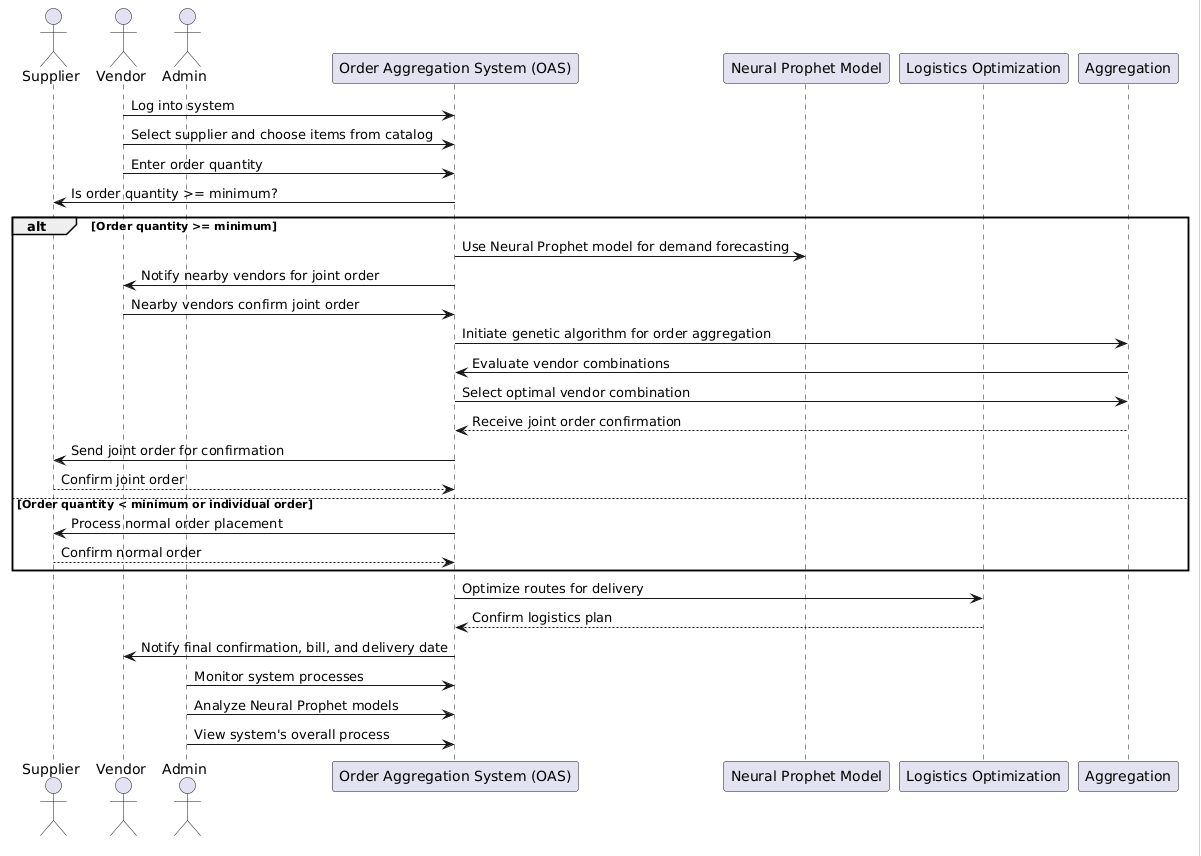
\includegraphics[width=1\textwidth]{Figures/Sequence Diagram.PNG}
    \caption{Sequence Diagram}
    \label{fig:sequence-diagram}
\end{figure}
\noindent Figure 4.2 illustrates the sequence of interactions between the key entities and components of the ASTRO Platform. This diagram provides a step-by-step view of how the system processes an order from initiation to delivery. It shows the flow of messages and the order in which they are exchanged, highlighting the interactions between the Supplier, Vendor, Admin, Order Aggregation System (OAS), Neural Prophet Model, and Logistics Optimization.
\subsection{Key Entities and Components}
\begin{itemize}
    \item \textbf{Supplier:} Manages product inventory and fulfills confirmed orders.
    \item \textbf{Vendor:} Places orders for products based on the demand forecast and minimum order requirements.
    \item \textbf{Admin:} Monitors the overall process, analyzes model performance, and reviews logistics planning.
    \item \textbf{Order Aggregation System (OAS):} Core system component that manages the flow of order requests, checks conditions, and coordinates with other components.
    \item \textbf{Neural Prophet Model:} A demand forecasting model that helps in predicting demand and evaluating whether joint orders would be beneficial.
    \item \textbf{Logistics Optimization:} Component responsible for optimizing delivery routes and managing the final logistics.
\end{itemize}
\subsection{Sequence of Interactions}

\begin{enumerate}
    \item \textbf{Login to System:} The Vendor initiates the sequence by logging into the system to access the product catalog, choose items, and place orders.
    \item \textbf{Select Supplier and Choose Items from Catalog:} The Vendor selects a supplier and items from the catalog, specifying the order quantity.
    \item \textbf{Order Quantity Check:} The Order Aggregation System (OAS) checks whether the order quantity meets the minimum order requirement.
          \begin{itemize}
              \item \textbf{If Order Quantity Meets Minimum Requirement:} The order is processed as a standard, individual order. The vendor confirms the order, and it proceeds to the delivery logistics phase.
              \item \textbf{If Order Quantity Is Below Minimum Requirement:} The OAS initiates steps to evaluate the feasibility of a joint order.
                    \begin{enumerate}
                        \item \textbf{Use Neural Prophet Model for Demand Forecasting:} The Neural Prophet Model is used to forecast demand and determine if combining orders from nearby vendors might help reach the minimum order quantity. This forecast provides data-driven insights into the order’s potential demand over time.
                        \item \textbf{Notify Nearby Vendors for Joint Order:} If the demand forecast suggests that a joint order is viable, the OAS sends notifications to nearby vendors, inviting them to participate in a joint order.
                        \item \textbf{Nearby Vendors Confirm Joint Order:} Other vendors respond to the joint order request. If they agree, the joint order process moves forward; otherwise, the initial vendor proceeds with an individual order.
                        \item \textbf{Initiate Genetic Algorithm for Order Aggregation:} The OAS employs a Genetic Algorithm to evaluate different combinations of vendors for the joint order, aiming to find an optimal mix that maximizes efficiency and meets the minimum order requirements.
                        \item \textbf{Evaluate Vendor Combinations:} The Genetic Algorithm component iterates through various vendor combinations to find the best possible aggregation. This ensures that the order is cost-effective and meets quantity requirements.
                        \item \textbf{Select Optimal Vendor Combination:} The system selects the optimal vendor combination for the joint order and proceeds to confirmation.
                        \item \textbf{Receive Joint Order Confirmation:} Once an optimal combination is selected, the OAS sends a joint order confirmation to all participating vendors. The joint order is now officially confirmed.
                    \end{enumerate}
          \end{itemize}
    \item \textbf{Order Processing and Final Confirmation:} For both joint and individual orders, the system notifies vendors of the final confirmation, bill, and delivery date.
    \item \textbf{Optimize Routes for Delivery:} The Logistics Optimization component optimizes delivery routes based on the confirmed orders, minimizing delivery time and cost by consolidating deliveries where possible.
    \item \textbf{Admin Activities:} The Admin monitors system processes and performance. Admin also reviews and analyzes the accuracy of Neural Prophet Model forecasts and evaluates system functionality, using insights to make improvements to the process.
\end{enumerate}
\section{Class Diagram}

A class diagram is a visual blueprint of a system in object-oriented programming, showcasing the classes, their attributes (properties), operations (methods), and the relationships between them. It’s like a map that reveals the building blocks and their connections, guiding the development and understanding of the system.

\subsection{Key Elements of Class Diagrams}
\begin{itemize}
    \item \textbf{Classes:} These are the fundamental building blocks, represented as rectangles with the class name inside. Each class encapsulates a specific concept or entity within the system, like "Customer" or "Order."
    \item \textbf{Attributes:} These define the data associated with a class, like "name" and "address" for the "Customer" class. They’re listed within the class rectangle, often with data types specified.
    \item \textbf{Operations:} These represent the actions a class can perform, like "placeOrder" or "calculateTotal" for the "Order" class. They’re shown as functions within the class rectangle, with their parameters and return values if applicable.
    \item \textbf{Relationships:} These depict the connections between classes, indicating how they interact with each other.
\end{itemize}
\begin{figure}[H]
    \centering
    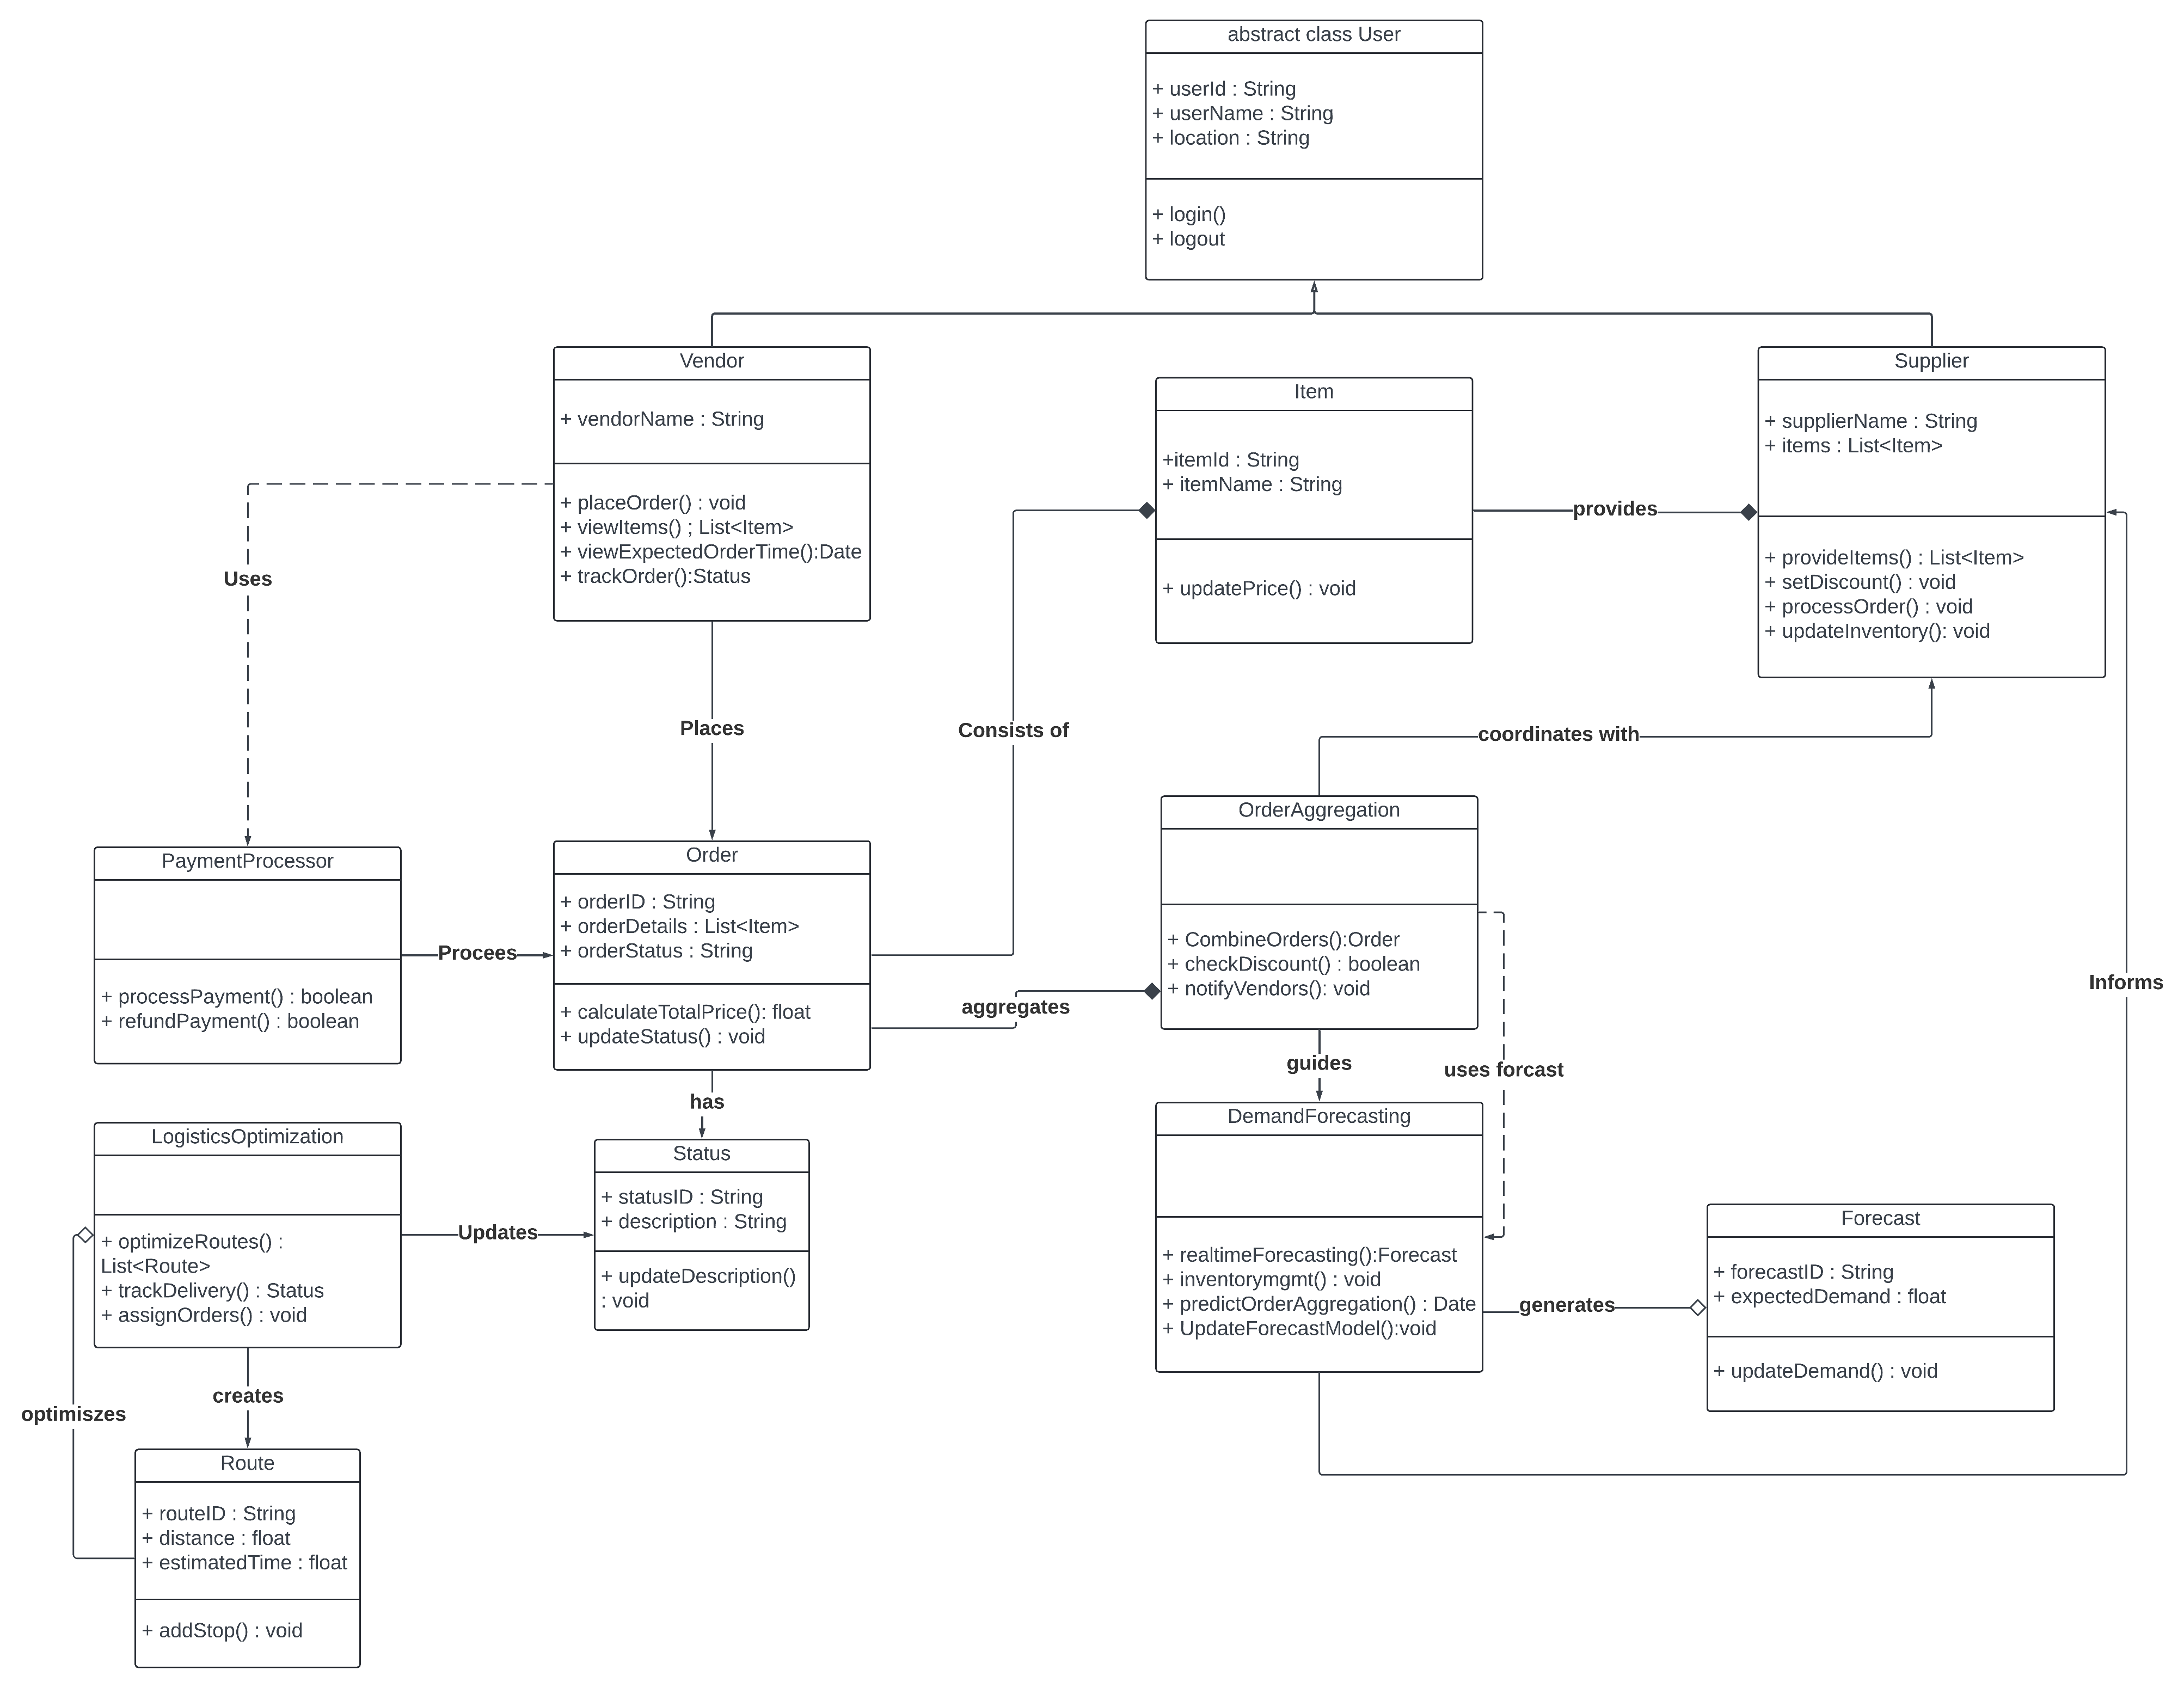
\includegraphics[width=1\textwidth]{Figures/Class Diagram.png}
    \caption{Class Diagram}
    \label{fig:class-diagram}
\end{figure}
\noindent Figure 4.3 illustrates the class diagram for the ASTRO Platform, showcasing the key classes and their relationships. This diagram provides a structural overview of the system, detailing the classes like User, Vendor, Supplier, Item, Order, Status, OrderAggregation, PaymentProcessor, LogisticsOptimization, DemandForecasting, and Forecast, along with their attributes and methods.
\subsection{Class Descriptions}

\begin{itemize}
    \item \textbf{User:} An abstract class representing a generic user with attributes like userId, userName, and location, along with methods login() and logout(). Inherited by Vendor and Supplier classes.

    \item \textbf{Vendor:} Represents a vendor who manages orders, with attributes such as vendorName and methods like placeOrder(), viewItems(), viewExpectedOrderTime(), and trackOrder(). Associated with Order and interacts with PaymentProcessor for payment handling.

    \item \textbf{Supplier:} Represents a supplier managing inventory with attributes like supplierName and items, and methods like provideItems(), setDiscount(), processOrder(), and updateInventory(). Coordinates with OrderAggregation and supplies items to the Item class.

    \item \textbf{Item:} Represents individual items with attributes like itemId and itemName, and a method updatePrice() to modify the item's price. Associated with Order as orders consist of multiple items.

    \item \textbf{Order:} Represents a customer order, including attributes orderID, orderDetails (list of items), and orderStatus, with methods calculateTotalPrice() and updateStatus(). Consists of multiple Item objects and is associated with Status.

    \item \textbf{Status:} Represents the order's current status with attributes statusID and description, and a method updateDescription() to modify the status description. Linked to Order to provide status details.

    \item \textbf{OrderAggregation:} Manages combined orders with methods CombineOrders(), checkDiscount(), and notifyVendors(). Coordinates with Supplier for order processing and informs DemandForecasting about aggregate demand.

    \item \textbf{PaymentProcessor:} Handles payments and refunds with methods processPayment() and refundPayment(). Interacts with Vendor for transaction management.

    \item \textbf{LogisticsOptimization:} Optimizes delivery routes with methods optimizeRoutes(), trackDelivery(), and assignOrders(), creating Route objects as part of logistics planning.

    \item \textbf{Route:} Represents a delivery route with attributes routeID, distance, and estimatedTime, and a method addStop() to add stops. Created by LogisticsOptimization.

    \item \textbf{DemandForecasting:} Predicts demand and manages inventory with methods like realtimeForecasting(), inventoryMgmt(), predictOrderAggregation(), and updateForecastModel(). Uses data from Forecast to guide order aggregation and inventory planning.

    \item \textbf{Forecast:} Provides demand forecasts with attributes forecastID and expectedDemand, and a method updateDemand(). Generated by DemandForecasting and used for planning inventory and order aggregation.
\end{itemize}
\subsection{Summary of Associations}
\begin{enumerate}
    \item Vendor places orders using Order and interacts with PaymentProcessor.
    \item Supplier provides Items to the system and coordinates with OrderAggregation for bulk orders.
    \item OrderAggregation combines orders and coordinates with Supplier, also informing DemandForecasting.
    \item DemandForecasting uses forecasts from Forecast to plan inventory and order aggregation.
    \item LogisticsOptimization creates Routes to optimize delivery.
\end{enumerate}

\subsection{Common Relationships}
\begin{itemize}
    \item \textbf{Association:} Shows a simple connection between two classes, like "Customer" has an "Order."
    \item \textbf{Aggregation:} A "has-a" relationship where one class (the whole) is made up of parts (the other class), like "Order" has "OrderItems."
    \item \textbf{Composition:} A stronger "has-a" relationship where the parts (the other class) cannot exist independently of the whole (one class), like "Car" has "Wheels."
    \item \textbf{Inheritance:} Shows a hierarchical relationship where one class (subclass) inherits properties and methods from another class (superclass), like "Employee" inherits from "Person."
\end{itemize}

\subsection{Benefits of Using Class Diagrams}
\begin{itemize}
    \item \textbf{Clarity:} They provide a visual representation of complex systems, making them easier to understand and communicate.
    \item \textbf{Communication:} They serve as a common language for developers, designers, and other stakeholders to agree on the system’s structure.
    \item \textbf{Analysis:} They help identify potential problems or inconsistencies in the system’s design before implementation.
    \item \textbf{Documentation:} They serve as a valuable reference for understanding and maintaining the system over time.
\end{itemize}

Where You Might Encounter Them
\begin{itemize}
    \item \textbf{Software Development:} Class diagrams are used throughout the software development lifecycle, from initial design to implementation and maintenance.
    \item \textbf{System Design:} They are crucial for modeling the architecture of complex systems, including web applications and enterprise software.
    \item \textbf{Documentation:} They are often included in technical documentation to provide a clear overview of the system’s structure.
\end{itemize}
\section{Use Case Diagram}
In the Unified Modeling Language (UML), a Use Case Diagram is a sort of behavioral diagram that depicts the interactions between various actors (users or external systems) and a system that is being studied. It offers a high-level perspective on how different entities use the features or functionalities of a system. A use case diagram’s main objective is to represent and illustrate the various ways users engage with a system and the results they receive.
\subsection{Key Elements of Use Case Diagrams}

\begin{itemize}
    \item \textbf{Use Case:} A use case is an example of a particular functionality or group of related functions that the system offers to its users, also known as actors. Use cases are designated to indicate a particular action or objective and are usually represented as ovals.

    \item \textbf{Actor:} An outside party interacting with the system is called an actor. Actors might be physical devices, other systems, or human actors. Stick figures are used to represent actors, who engage with the system by taking part in one or more use cases.

    \item \textbf{System Boundary:} Depicted as a box, the system boundary establishes the parameters of the system and demarcates its external participants. Actors reside outside the system boundaries, whereas use cases exist inside it.

    \item \textbf{Association:} Associations are shown as lines joining actors to use cases. These lines show that an actor participates in or communicates with a certain use case. Associations serve as a channel of communication between the use case and the actor.

    \item \textbf{Include Relationship:} An include relationship shows that one use case incorporates the functionality of another use case. It is represented by a dashed arrow. It suggests that the behavior of the base use case includes the added use case.

    \item \textbf{Extend Relationship:} An extended connection shows that, under certain circumstances, one use case can extend the behavior of another use case. It is represented by a dashed arrow with an open arrowhead. It suggests that the expanding use case is called upon under particular circumstances and is optional.

\end{itemize}
Some use cases might not include interactions with a particular actor; instead, they might represent system-wide operations or processes. We call these use cases for the system.

\subsection{Value of Use Case Diagrams}

Use Case Diagrams are valuable tools for:
\begin{itemize}
    \item \textbf{Communication:} Use case diagrams offer a visual representation that helps stakeholders—developers, designers, and non-technical stakeholders—communicate with one other.
    \item \textbf{Requirements Analysis:} By recognizing and recording user-system interactions, they aid in the elicitation and clarification of system requirements.
    \item \textbf{System Design:} The architecture and user interfaces of the system are designed using use case diagrams as a guide.
    \item \textbf{Testing:} By figuring out scenarios in which users engage with the system, they can be used to generate test cases.
    \item \textbf{Project Planning:} By highlighting important features and their relationships, use case diagrams can help with project planning.
\end{itemize}
\begin{figure}[H]
    \centering
    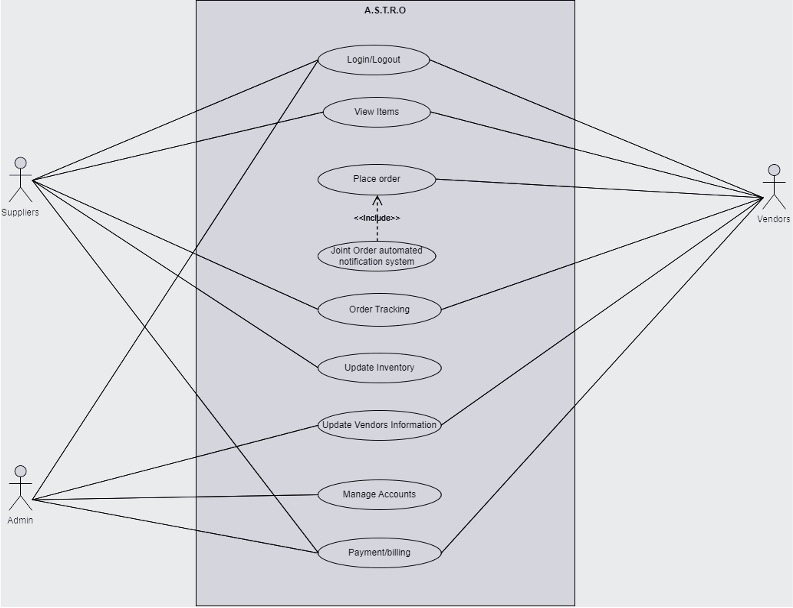
\includegraphics[width=1\textwidth]{Figures/Use case diagram.jpg}
    \caption{Use Case Diagram}
    \label{fig:use-case-diagram}
\end{figure}
\noindent Figure 4.4 illustrates the use case diagram for the ASTRO Platform, showcasing the interactions between the actors (Suppliers, Vendors, and Admin) and the system. This diagram provides a high-level view of the functionalities available to each actor and how they interact with the system to place orders, manage inventory, track orders, and perform administrative tasks.
\subsection{Actors}

\begin{enumerate}
    \item \textbf{Suppliers:}
          \begin{itemize}
              \item Responsible for providing inventory or items for the system.
              \item Has access to most functions related to orders, inventory, and tracking.
          \end{itemize}

    \item \textbf{Vendors:}
          \begin{itemize}
              \item Likely responsible for purchasing or receiving items in the system.
              \item Similar to Suppliers, has access to most functions, especially those related to placing orders, notifications, and tracking.
          \end{itemize}

    \item \textbf{Admin:}
          \begin{itemize}
              \item Responsible for overall management, including accounts and billing.
              \item Has the ability to manage vendor information and accounts in addition to other functionalities.
          \end{itemize}
\end{enumerate}
\subsection{Use Cases}

\begin{enumerate}
    \item \textbf{Login/Logout:}
          \begin{itemize}
              \item All users (Suppliers, Vendors, and Admin) can log in and log out of the system, indicating that authentication is a standard feature.
          \end{itemize}

    \item \textbf{View Items:}
          \begin{itemize}
              \item Suppliers and Vendors have access to this use case, allowing them to view items available in the system, possibly for ordering or tracking purposes.
          \end{itemize}

    \item \textbf{Place Order:}
          \begin{itemize}
              \item Both Suppliers and Vendors can place orders in the system, which might include ordering goods or services. This use case includes an include relationship to the Joint Order Automated Notification System use case, meaning that when an order is placed, an automated notification system is triggered.
          \end{itemize}

    \item \textbf{Joint Order Automated Notification System:}
          \begin{itemize}
              \item An included use case for the Place Order use case.
              \item This automated system sends notifications for joint orders, possibly to inform both Suppliers and Vendors of order status or details.
          \end{itemize}

    \item \textbf{Order Tracking:}
          \begin{itemize}
              \item Both Suppliers and Vendors can track the status of their orders through the system, giving them visibility into order fulfillment stages.
          \end{itemize}

    \item \textbf{Update Inventory:}
          \begin{itemize}
              \item This use case allows both Suppliers and Vendors to update inventory information, which could involve adding, editing, or removing items based on stock levels or requirements.
          \end{itemize}

    \item \textbf{Update Vendors Information:}
          \begin{itemize}
              \item Accessible by all actors, including Admin.
              \item This use case allows updating information related to Vendors, which could involve updating contact details, address, or other essential information.
          \end{itemize}

    \item \textbf{Manage Accounts:}
          \begin{itemize}
              \item Specific to the Admin, who has control over managing accounts in the system.
              \item This might involve user account creation, permissions, and other administrative tasks.
          \end{itemize}

    \item \textbf{Payment/Billing:}
          \begin{itemize}
              \item Only the Admin has access to this functionality, likely responsible for handling the financial aspects of transactions in the system, including processing payments and issuing bills.
          \end{itemize}
\end{enumerate}
\subsection{Relationships}

\begin{itemize}
    \item \textbf{Include Relationship:}
          The Place Order use case includes the Joint Order Automated Notification System, meaning that this automated notification is a required part of placing an order. This might help keep all parties informed about order updates.


    \item \textbf{System Boundary:}
          The shaded box labeled A.S.T.R.O represents the system boundary, meaning all the use cases within this box are functionalities provided by the A.S.T.R.O system.

\end{itemize}